%%%%%%%%%%%%%%%%%%%%%%%%%%%%%%%%%%%%%%%%%%%%%%%%%%%%%%%%%%%%%%%%%%%%%%
% Problem statement
\begin{statement}[
  problempoints=100,
  timelimit=1 second,
  memorylimit=1024 MiB,
]{Ministarstvo}

After a successful career in a party we won't name, Pero got a job at the Ministry of Tourism. Pero oversees a network of $N$ cities, labeled with numbers from $1$ to $N$, where there is exactly one, one-way road between each pair of cities. In order to increase revenue, he has decided to introduce permits for traffic. Pero would prefer to introduce a special permit for each road, but that would alert his superiors. Therefore, he will introduce $K$ different permits, labeled from $1$ to $K$, and possession of a specific permit will be required to travel on each road.

To still ensure substantial revenue, Pero will settle for the following property.

\begin{itemize}
\item For each city $v$, there is some city $u$, such that it is not possible to travel from city $v$ to city $u$ with just one permit.
\end{itemize} 

Pero asks for your help to determine the minimum $K$ such that there exists an assignment of permits with the desired property, if such an assignment exists! If no such assignment exists, output \texttt{-1}. 

%%%%%%%%%%%%%%%%%%%%%%%%%%%%%%%%%%%%%%%%%%%%%%%%%%%%%%%%%%%%%%%%%%%%%%
% Input
\subsection*{Input}

The first line contains a natural number $N$.

The $i$-th of the following $N$ lines contains $N$ numbers $a_{i, j}$ where $a_{i, j} = 1$ if there is a road from city $i$ to city $j$. Note that $a_{i, i} = 0$ and for $i \neq j$, exactly one of the numbers $a_{i, j}$ and $a_{j, i}$ is non-zero. 

%%%%%%%%%%%%%%%%%%%%%%%%%%%%%%%%%%%%%%%%%%%%%%%%%%%%%%%%%%%%%%%%%%%%%%
% Output
\subsection*{Output}

If there is no assignment with the desired property, output \texttt{-1} in the first and only line.

Otherwise, output the minimum natural number $K$ in the first line.

In the following $N$ lines, output the description of the assignment.

In the $i$-th line, output $N$ numbers $b_{i, j}$ where if $a_{i, j} = 0$, then $b_{i, j} = 0$, otherwise $1 \leq b_{i, j} \leq K$ indicating which permit is required for traveling on that road. 

%%%%%%%%%%%%%%%%%%%%%%%%%%%%%%%%%%%%%%%%%%%%%%%%%%%%%%%%%%%%%%%%%%%%%%
% Scoring
\subsection*{Scoring}

In all subtasks, $2 \leq N \leq 1000$. In each subtask, $15\%$ of the points come from only deciding whether such an assignment exists or not. For these points, if you don't output \texttt{-1}, you need to output some assignment, but it doesn't have to satisfy Pero's desired property. 

{\renewcommand{\arraystretch}{1.4}
  \setlength{\tabcolsep}{6pt}
  \begin{tabular}{ccl}
   Subtask & Score & Constraints \\ \midrule
    1 & 20 & $N \leq 5$  \\
    2 & 80 & No additional constraints. \\
\end{tabular}}

%%%%%%%%%%%%%%%%%%%%%%%%%%%%%%%%%%%%%%%%%%%%%%%%%%%%%%%%%%%%%%%%%%%%%%
% Examples
\subsection*{Examples}
\begin{tabularx}{\textwidth}{X'X'X}
\sampleinputs{test/ministarstvo.dummy.in.1}{test/ministarstvo.dummy.out.1} &
\sampleinputs{test/ministarstvo.dummy.in.2}{test/ministarstvo.dummy.out.2} &
\sampleinputs{test/ministarstvo.dummy.in.3}{test/ministarstvo.dummy.out.3}
\end{tabularx}

\textbf{Explanation for the third sample test:}\\

Roads requiring the first permit are marked in red, the second permit in blue, and the third permit in green.

From city $1$, it is not possible to reach city $3$ using just one permit.

From city $2$, it is not possible to reach city $1$ using just one permit.

From city $3$, it is not possible to reach city $2$ using just one permit.

From city $4$, it is not possible to reach city $1$ using just one permit.


\centering
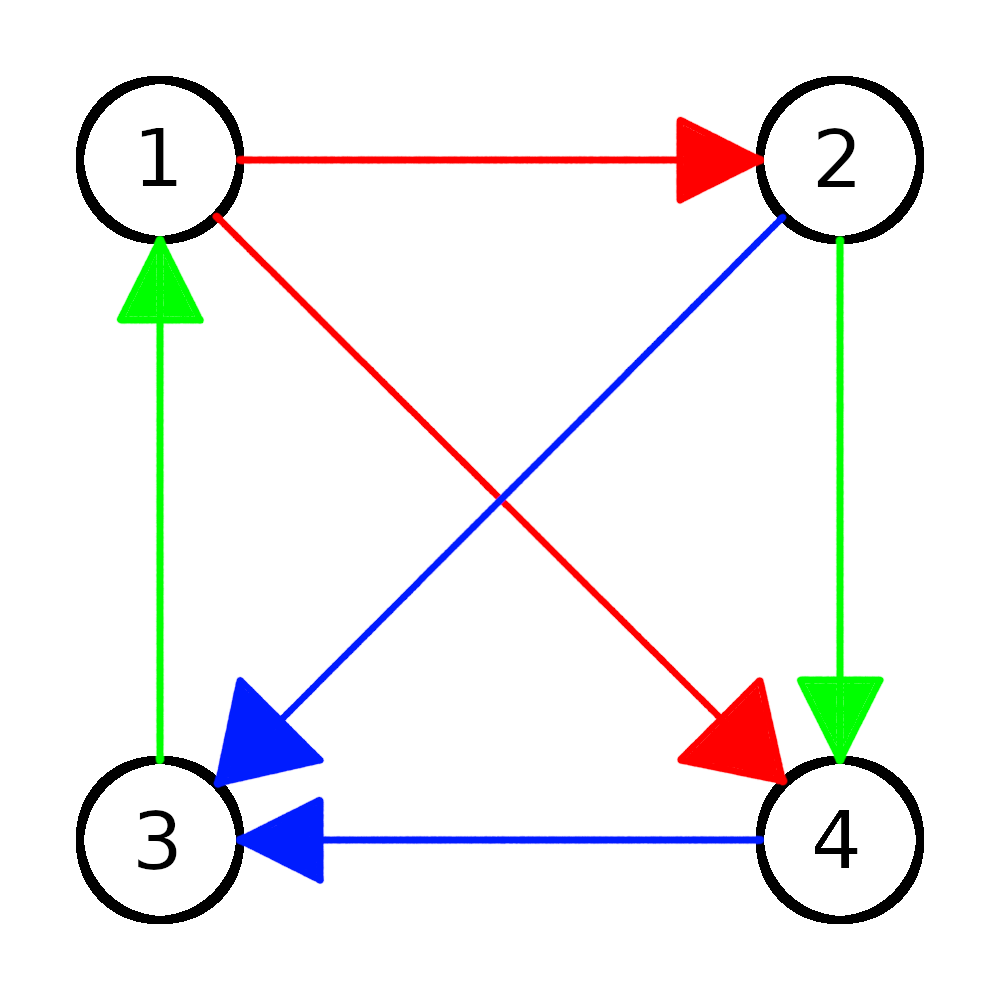
\includegraphics[scale=1]{pic/skcia3.png}
  
%%%%%%%%%%%%%%%%%%%%%%%%%%%%%%%%%%%%%%%%%%%%%%%%%%%%%%%%%%%%%%%%%%%%%%
% We're done
\end{statement}